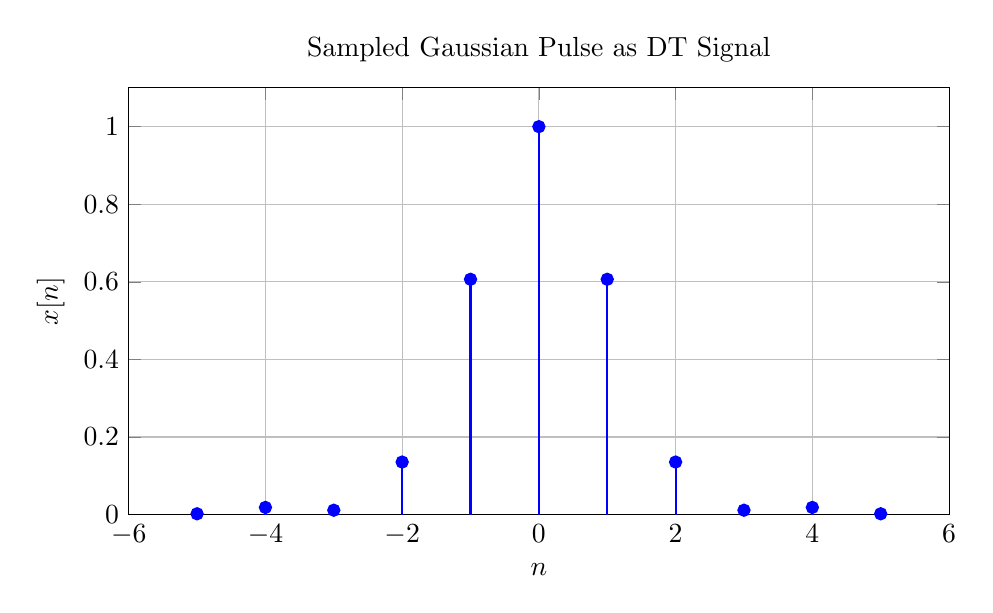
\begin{tikzpicture}
	\begin{axis}[
		title={Sampled Gaussian Pulse as DT Signal},
		xlabel={$n$},
		ylabel={$x[n]$},
		xmin=-6, xmax=6,
		ymin=0, ymax=1.1,
		grid=major,
		width=12cm,
		height=7cm,
		]
		\addplot[
		ycomb,
		blue,
		thick,
		mark=*,
		mark options={fill=blue},
		]
		coordinates {
			(-5,0.0019) (-4,0.0183) (-3,0.0111) (-2,0.1353)
			(-1,0.6065) (0,1) (1,0.6065) (2,0.1353)
			(3,0.0111) (4,0.0183) (5,0.0019)
		};
	\end{axis}
\end{tikzpicture}
